%
% results.tex
% Copyright (C) 2021 by Krish Kabra, <krish@kabra.com>.
%

\chapter{Results} \label{chap:methods}

\begin{figure}[t]
    \centering
    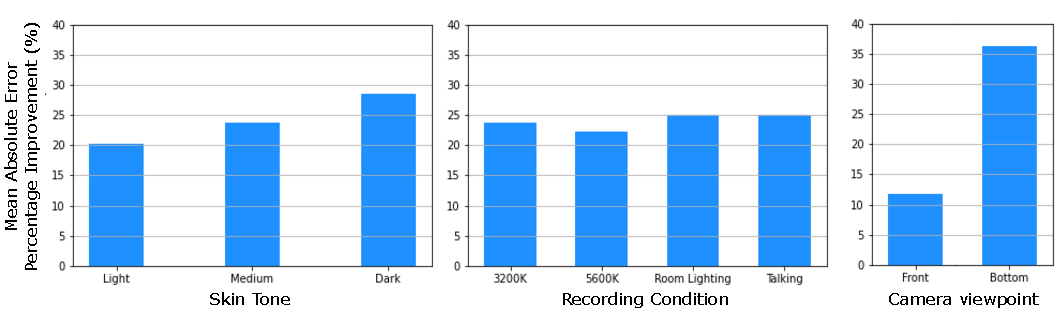
\includegraphics[width=\linewidth]{include/fig-barplot-MAE-percentage.pdf}
    \caption{\textbf{The proposed method achieves significant performance gains for all skin tones in a manner that mitigates skin tone bias.} The MAE percentage improvement with respect to the baseline facial aggregation method shows significant performance gains across all skin tones, recording conditions, and camera viewpoints. Specifically, the proposed method achieves the largest performance gain for dark skin tones, followed by medium and light skin tones respectively.}
    \label{fig:barplot}
\end{figure}

\begin{table}[]
\begin{center}
\scalebox{0.66}{
\begin{tabular}{c|c|ccccccccccccc}
\multirow{3}{3.5cm}{\begin{tabular}[c]{@{}c@{}}Denoising \\ Method\end{tabular}} & \multirow{3}{*}{Statistic} & \multicolumn{13}{c}{Front} \\ \cline{3-15} 
 &  & \multicolumn{3}{c|}{3200K} & \multicolumn{3}{c|}{5600K} & \multicolumn{3}{c|}{Room Lighting} & \multicolumn{3}{c|}{Talking} & \multirow{2}{*}{Overall} \\ \cline{3-14}
 &  & Light & Med. & \multicolumn{1}{c|}{Dark} & Light & Med. & \multicolumn{1}{c|}{Dark} & Light & Med. & \multicolumn{1}{c|}{Dark} & Light & Med. & \multicolumn{1}{c|}{Dark} &  \\ \hline
\multirow{3}{3.5cm}{Facial Aggregation} & MAE & 7.88 & 9.88 & \multicolumn{1}{c|}{13.10} & 8.25 & 8.28 & \multicolumn{1}{c|}{\textbf{12.49}} & 9.29 & 8.14 & \multicolumn{1}{c|}{13.54} & 10.32 & 11.17 & \multicolumn{1}{c|}{14.00} & 10.01 \\
 & SDE & 9.30 & 10.45 & \multicolumn{1}{c|}{15.08} & 9.26 & 9.06 & \multicolumn{1}{c|}{13.10} & 11.70 & 7.30 & \multicolumn{1}{c|}{13.22} & 10.75 & 10.87 & \multicolumn{1}{c|}{16.72} & 10.76 \\
 & R & 0.29 & 0.20 & \multicolumn{1}{c|}{\textbf{0.02}} & 0.25 & \textbf{0.39} & \multicolumn{1}{c|}{0.01} & 0.32 & 0.35 & \multicolumn{1}{c|}{0.02} & 0.27 & 0.18 & \multicolumn{1}{c|}{\textbf{0.17}} & 0.24 \\ \hline
\multirow{3}{3.5cm}{SNR Weighting} & MAE & 7.10 & 11.62 & \multicolumn{1}{c|}{13.52} & 7.72 & 12.51 & \multicolumn{1}{c|}{15.14} & 8.93 & 9.27 & \multicolumn{1}{c|}{17.19} & 9.95 & 11.74 & \multicolumn{1}{c|}{13.02} & 10.97 \\
 & SDE & 7.86 & 11.44 & \multicolumn{1}{c|}{12.44} & 8.59 & 11.83 & \multicolumn{1}{c|}{12.80} & 10.34 & 9.57 & \multicolumn{1}{c|}{16.09} & 11.29 & 12.28 & \multicolumn{1}{c|}{14.16} & 11.18 \\
 & R & 0.39 & 0.11 & \multicolumn{1}{c|}{-0.03} & 0.43 & 0.13 & \multicolumn{1}{c|}{-0.17} & 0.33 & 0.36 & \multicolumn{1}{c|}{-0.05} & 0.36 & 0.20 & \multicolumn{1}{c|}{0.15} & 0.21 \\ \hline
\multirow{3}{3.5cm}{\textit{Diverse R-PPG (Proposed Method)}} & MAE & \textbf{6.32} & \textbf{7.91} & \multicolumn{1}{c|}{\textbf{12.40}} & \textbf{7.61} & \textbf{7.96} & \multicolumn{1}{c|}{13.49} & \textbf{8.84} & \textbf{7.17} & \multicolumn{1}{c|}{\textbf{12.95}} & \textbf{8.59} & \textbf{8.12} & \multicolumn{1}{c|}{\textbf{12.00}} & \textbf{8.81} \\
 & SDE & \textbf{6.81} & \textbf{6.27} & \multicolumn{1}{c|}{\textbf{10.39}} & \textbf{7.95} & \textbf{7.16} & \multicolumn{1}{c|}{\textbf{10.39}} & \textbf{7.19} & \textbf{5.94} & \multicolumn{1}{c|}{\textbf{8.71}} & \textbf{7.92} & \textbf{6.46} & \multicolumn{1}{c|}{\textbf{9.84}} & \textbf{7.50} \\
 & R & \textbf{0.53} & \textbf{0.28} & \multicolumn{1}{c|}{-0.05} & \textbf{0.44} & 0.37 & \multicolumn{1}{c|}{\textbf{0.09}} & \textbf{0.36} & \textbf{0.42} & \multicolumn{1}{c|}{\textbf{0.12}} & \textbf{0.42} & \textbf{0.52} & \multicolumn{1}{c|}{0.01} & \textbf{0.32} \\ \hline
 \hline
 & \multicolumn{1}{l|}{} & \multicolumn{13}{c}{Bottom} \\ \cline{3-15} 
 & \multicolumn{1}{l|}{} & \multicolumn{3}{c|}{3200K} & \multicolumn{3}{c|}{5600K} & \multicolumn{3}{c|}{Room Lighting} & \multicolumn{3}{c|}{Talking} & \multicolumn{1}{l}{\multirow{2}{*}{Overall}} \\ \cline{3-14}
 & \multicolumn{1}{l|}{} & Light & Med. & \multicolumn{1}{c|}{Dark} & Light & Med. & \multicolumn{1}{c|}{Dark} & Light & Med. & \multicolumn{1}{c|}{Dark} & Light & Med. & \multicolumn{1}{c|}{Dark} & \multicolumn{1}{l}{} \\ \hline
\multirow{3}{3.5cm}{Facial Aggregation} & MAE & 4.77 & 8.51 & \multicolumn{1}{c|}{11.92} & 6.52 & 7.52 & \multicolumn{1}{c|}{19.25} & 9.20 & 9.17 & \multicolumn{1}{c|}{14.82} & 11.75 & 11.66 & \multicolumn{1}{c|}{15.80} & 10.07 \\
 & SDE & 7.41 & 9.73 & \multicolumn{1}{c|}{15.42} & 8.05 & 10.52 & \multicolumn{1}{c|}{20.21} & 10.68 & 12.62 & \multicolumn{1}{c|}{21.15} & 12.46 & 12.22 & \multicolumn{1}{c|}{19.28} & 12.27 \\
 & R & 0.69 & 0.35 & \multicolumn{1}{c|}{0.32} & 0.40 & 0.53 & \multicolumn{1}{c|}{0.11} & 0.33 & 0.25 & \multicolumn{1}{c|}{0.18} & 0.19 & 0.17 & \multicolumn{1}{c|}{0.10} & 0.30 \\ \hline
\multirow{3}{3.5cm}{SNR Weighting} & MAE & 6.13 & 9.24 & \multicolumn{1}{c|}{13.07} & 6.67 & 10.08 & \multicolumn{1}{c|}{16.39} & 7.81 & 7.92 & \multicolumn{1}{c|}{15.33} & 10.41 & 11.77 & \multicolumn{1}{c|}{12.90} & 9.99 \\
 & SDE & 8.86 & 10.96 & \multicolumn{1}{c|}{16.80} & 8.67 & 11.42 & \multicolumn{1}{c|}{18.31} & 9.63 & 8.59 & \multicolumn{1}{c|}{21.89} & 11.09 & 12.05 & \multicolumn{1}{c|}{14.63} & 11.78 \\
 & R & 0.57 & 0.36 & \multicolumn{1}{c|}{0.32} & 0.45 & 0.28 & \multicolumn{1}{c|}{0.23} & 0.39 & 0.32 & \multicolumn{1}{c|}{0.03} & 0.28 & 0.20 & \multicolumn{1}{c|}{\textbf{0.18}} & 0.29 \\ \hline
\multirow{3}{3.5cm}{\textit{Diverse R-PPG (Proposed Method)}} & MAE & \textbf{4.31} & \textbf{5.10} & \multicolumn{1}{c|}{\textbf{7.13}} & \textbf{4.47} & \textbf{5.88} & \multicolumn{1}{c|}{\textbf{6.82}} & \textbf{5.86} & \textbf{5.95} & \multicolumn{1}{c|}{\textbf{6.61}} & \textbf{8.12} & \textbf{8.57} & \multicolumn{1}{c|}{\textbf{10.83}} & \textbf{6.43} \\
 & SDE & \textbf{5.01} & \textbf{4.15} & \multicolumn{1}{c|}{\textbf{7.48}} & \textbf{4.50} & \textbf{5.04} & \multicolumn{1}{c|}{\textbf{7.34}} & \textbf{5.51} & \textbf{4.95} & \multicolumn{1}{c|}{\textbf{7.67}} & \textbf{6.91} & \textbf{6.68} & \multicolumn{1}{c|}{\textbf{9.30}} & \textbf{5.86} \\
 & R & \textbf{0.72} & \textbf{0.66} & \multicolumn{1}{c|}{\textbf{0.64}} & \textbf{0.65} & \textbf{0.57} & \multicolumn{1}{c|}{\textbf{0.59}} & \textbf{0.54} & \textbf{0.51} & \multicolumn{1}{c|}{\textbf{0.54}} & \textbf{0.46} & \textbf{0.38} & \multicolumn{1}{c|}{0.14} & \textbf{0.54} \\ 
\end{tabular}}
\end{center}
\caption{\textbf{The proposed method achieves state-of-the-art performance across skin tones, recording conditions and camera viewpoints.} The numbers bolded represent the best statistic across the 3 methods for the particular category and metric. For the bottom camera viewpoint, the skin tone bias is almost completely eliminated for non-talking recording conditions.}
\label{tab:results}
\end{table}
    
% \section{Statistical analysis}

To quantitatively assess the performance of the proposed method against the facial aggregation and SNR weighting benchmark techniques, we perform remote HR estimation for across the 472 videos contained in the VITAL dataset. HR estimation is carried out for windows of duration 20 seconds, with an overlap of 10 seconds. 

Table~\ref{tab:results} shows the comprehensive results of the benchmark and proposed methods categorized by skin tone, recording condition, and camera viewpoint. Figure~\ref{fig:barplot} highlights the significant performance gain of the proposed method over the benchmark facial aggregation method with respect to skin tone, recording condition, and camera viewpoint, by fixing each category. 

The following statistical metrics are used: (i) Mean Absolute Error (MAE), (ii) Standard deviation of the error (SDE) and the correlation coefficient (r), between the estimated R-PPG HR and the ground truth PPG HR in a given 20 second window. We note that there exists an offset between the ground truth PPG waveform and predicted R-PPG waveform due to both experimental delay between the recorded video and captured vital signs as well as biological delay between the BVP signal from the finger and face. Nevertheless, due to the long window size within which the HR is determined, we suspect the delays are negligible. 

\section{Skin tone performance}

For all three methods, performance degrades from light to dark skin. The facial aggregation approach obtains a MAE of 8.45, 9.34, and 14.38 bpm for light, medium and dark skin tone subjects, resulting in an overall average performance of 10.04 bpm. When comparing the facial aggregation results to the SNR weighting approach, the SNR weighting approach achieves a MAE improvement of 4.6\% (+0.39 bpm) for light skin tones, and a successive MAE degradation of -13.1\% (-1.22 bpm) and -1.7\% (-0.24 bpm) is obtained for medium and dark skin tones respectively. Hence, on a skin tone diverse dataset such as VITAL, this leads to a comparative decrease in overall performance of 0.04\% (-0.44 bpm). In contrast, the proposed method shows significant improvement across all skin tones when compared to the facial aggregation method, with a MAE improvement of 20.2\% (+1.71 bpm), 23.7\% (+2.22) bpm and 28.5\% (+4.11 bpm) obtained for light, medium and dark skin tones respectively. Consequently, the overall performance of the proposed method on the VITAL dataset improves by 0.24\% (+2.42 bpm), and the bias across skin tones is reduced from 5.93 bpm MAE difference between light and dark skin tones to 3.53 bpm. Therefore, the proposed method helps mitigate skin tone bias leading to a more fair R-PPG system. Nevertheless, the bias is still non-zero.  

\section{Recording condition performance}

Each of the three methods performs best in the warm lighting condition, and worst in the room lighting condition. The facial aggregation method shows an MAE of 8.85, 9.35, and 10.02 bpm across the warm, cool and room lighting conditions respectively, while the SNR weighting method shows an MAE of 9.67, 10.71, and 10.14 bpm across the lighting conditions respectively. This is a performance degradation of -9.2\% (-0.82 bpm), -14.5\% (1.36 bpm), and -1.1\% (-0.12 bpm) across the lighting conditions respectively. The proposed methods shows significant improvement across the lighting conditions, with a MAE of 6.75, 7.27, and 7.52 bpm across the warm, cool and room lighting conditions respectively. This is a performance improvement of 23.7\% (2.10 bpm), 22.3\% (2.08 bpm), and 25.0\% (2.50 bpm) across the lighting conditions respectively. This improvement also results in a reduced illumination bias from a difference of 1.17 bpm between warm and room lighting conditions to 0.77 bpm. 

The performance on the ‘talking’ activity is worse as compared to that on other scene conditions for all three methods. The SNR weighting method shows a MAE improvement of 4.4\% (+0.52 bpm) over the facial aggregation benchmark. However, the proposed method shows a larger improvement of 25.0\% (+3.01 bpm) when compared to the facial aggregation benchmark. 

\section{Camera viewpoint performance}

For all three methods, the bottom camera viewpoint performs the best. The facial aggregation method shows a MAE of 10.01 bpm for the front setting, and 10.07 bpm for the bottom setting, the SNR weighting method shows MAE of 10.97 bpm and 9.99 bpm, and the proposed method shows a MAE of 8.81 bpm and 6.43 bpm. The performance improvement of the proposed method corresponds to 11.8\% (+1.20 bpm) and 36.2\% (+3.64 bpm) for the front and bottom viewpoints respectively.

